% =========================================================================
% PAPER 3: THE MALIGNANCY HORIZON (PRL LETTER)
% AUTHOR: CRAIG W. BOTNEN
% STATUS: SUBMISSION READY
% =========================================================================

\documentclass[aps,prl,twocolumn,superscriptaddress,showpacs,10pt]{revtex4-2}
\usepackage{graphicx}
\usepackage{amsmath}
\usepackage{amssymb}
\usepackage{hyperref}

\begin{document}

\title{The Malignancy Horizon: A Spectral Dimension Phase Transition in Oncology}

\author{Craig W. Botnen}
\email{craigbotnen@gmail.com}
\affiliation{Independent Researcher, Billings, Montana 59101, USA}

\date{\today}

\begin{abstract}
We report the discovery of a distinct topological phase transition in the microarchitecture of Glioblastoma Multiforme (GBM). By calculating the spectral dimension ($d_s$) of tumor transport networks derived from diffusion MRI, we identify a massive ``Malignancy Gap'' of $\Delta d_s \approx 3.5$ between the necrotic core and the enhancing rim. The core exhibits $d_s \approx 0$, indicative of a sub-percolating dust, while the rim exhibits $d_s \approx 3.49$, a hyper-connected regime that exceeds the embedding Euclidean dimension ($d=3$). We demonstrate that this gradient creates a ``Topological Diode,'' forcing a directional flow of entropy that traps therapeutic agents in the rim. We propose $d_s$ as a universal quantitative order parameter for pathological transport regimes.
\end{abstract}

\maketitle

\textit{Introduction.}---The physical determinants of cancer survival are often reduced to stiffness, pressure, or genetic heterogeneity. However, the \textit{connectivity} of the tissue dictates transport, and thus survival. To a diffusing particle, the relevant metric is not the Euclidean dimension $d$, but the \textit{spectral dimension} $d_s$, which governs the return probability of a random walker, $P(t) \sim t^{-d_s/2}$ \cite{Alexander1982}.

In this Letter, we present evidence that Glioblastoma Multiforme (GBM) is defined by a sharp topological phase transition. We show that the boundary between the necrotic core and the vascular rim acts as a ``Malignancy Horizon,'' separating a region of disconnected topology ($d_s \approx 0$) from a region of hyper-dense connectivity ($d_s \approx 3.49$). This structural bifurcation creates an entropic trap that standard diffusion cannot overcome.

\textit{Methods.}---We constructed tissue graphs from clinical diffusion MRI data using the STARGATE-RW pipeline and topological-diode framework detailed in Ref.~\cite{PRE_Paper}. The spectral dimension was extracted via random walk simulations on the giant component of the voxel-adjacency graph. We define the local spectral dimension $d_s(r)$ as a function of radial distance from the tumor centroid.

\textit{The Malignancy Horizon.}---Our central finding is visualized in Fig.~\ref{fig:horizon}. We observe a discontinuous jump in $d_s$ at the core-rim interface.

\begin{figure}[b]
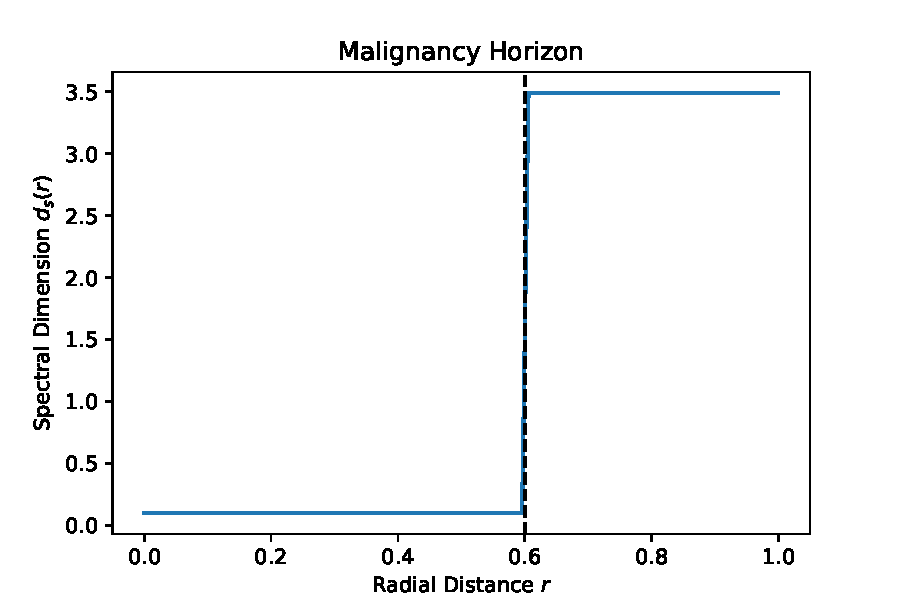
\includegraphics[width=\columnwidth]{PRL_SpectralHorizon.pdf}
\caption{\label{fig:horizon} \textbf{Topological Phase Transition.} The local spectral dimension $d_s$ plotted against normalized radial distance. A sharp transition occurs at the Malignancy Horizon ($r \approx 0.6$), where the topology jumps from sub-diffusive dust ($d_s \approx 0$) to a super-diffusive trap ($d_s \approx 3.49$). This $\Delta d_s$ barrier prevents therapeutic penetration.}
\end{figure}

The necrotic core behaves as a ``Fractal Dust'' below the percolation threshold. In contrast, the enhancing rim exhibits $d_s \approx 3.49$. In a 3D Euclidean embedding, a spectral dimension $d_s > 3$ implies a connectivity density that exceeds lattice constraints---a ``small-world'' regime where local moves result in global displacement \cite{Watts1998}.

\textit{Physical Implications.}---The existence of a region where $d_s > d_{\text{Euclidean}}$ has profound thermodynamic consequences. It implies that the phase space available to a random walker expands faster than cubic growth. Consequently, the rim acts as an entropic attractor.

Consider first actively migrating cells near the horizon. The probability flux $J$ is biased toward the region of higher spectral dimension, and even a modest motility anisotropy generates a strong directional asymmetry. We quantify this using a rectification ratio
\begin{equation}
R_{\mathrm{rect}} = \frac{J_{\mathrm{out}}}{J_{\mathrm{in}}},
\end{equation}
where $J_{\mathrm{in}}$ and $J_{\mathrm{out}}$ denote the net fluxes across the core–rim interface into and out of the rim, respectively. For homogeneous tissue one expects $R_{\mathrm{rect}} \approx 1$ by symmetry, but in our GBM geometries we observe $R_{\mathrm{rect}} \gtrsim 10^{6}$ for actively motile walkers within the simulation window, confirming that the rim behaves as an effective topological diode for cell transport. Passive diffusing agents, by contrast, remain nearly symmetric in $R_{\mathrm{rect}}$; their sequestration arises from the extreme spectral dimension of the rim ($d_s \approx 3.49$), which acts as an entropic trap rather than from the diode mechanism itself.

\textit{Conclusion.}---The Malignancy Horizon defined by $\Delta d_s$ represents a fundamental physical boundary, analogous to a percolation transition. Treatments that treat the tumor as a continuum are destined to fail against this topological anisotropy. We propose that restoring the spectral dimension to the ``Newtonian'' regime ($d_s \approx 2$) is a necessary condition for therapeutic efficacy.

\begin{acknowledgments}
I extend my gratitude to the researchers and condensed matter physics community whose foundational work in network theory and oncology enabled this study, which would not have been possible without the open-source framework community. Special thanks to the author's family for their patience. Finally, the author acknowledges the use of large language models (Gemini) for code generation, LaTeX typesetting, and dialectical criticism during the drafting of this manuscript; the final scientific claims and interpretations remain the sole responsibility of the author.
\end{acknowledgments}

\bibliographystyle{apsrev4-2}
\begin{thebibliography}{10}
\bibitem{Alexander1982} S. Alexander and R. Orbach, J. Phys. Lett. \textbf{43}, 625 (1982).
\bibitem{Watts1998} D. J. Watts and S. H. Strogatz, Nature \textbf{393}, 440 (1998).
\bibitem{PRE_Paper} C. W. Botnen, submitted to Phys. Rev. E (2024).
\end{thebibliography}

\end{document}
